\documentclass[12pt, oneside]{article}
 
% PKG : police du rapport 
\usepackage[sfdefault]{roboto} 
\usepackage[T1]{fontenc}
\usepackage[utf8]{inputenc}

%%%%%%%%%%%%%%%%%%%%%%%%%%%%%%%%%%%%%%%%%%%%%%%%%%%%%%%%%%%%%%%%%%%%%%%%
%%%%%%%%%%%%%%%%%%%%%%%%%%% ZONE A CHANGER %%%%%%%%%%%%%%%%%%%%%%%%%%%%%
%%%%%%%%%%%%%%%%%%%%%%%%%%%%%%%%%%%%%%%%%%%%%%%%%%%%%%%%%%%%%%%%%%%%%%%%

\newcommand{\type}{05/06/2018}	% Date
\newcommand{\auteur}{\item Jérémy Martin
				      \item Nicolas Fontaine}	% Auteur du compte-rendu
			 
%%%%%%%%%%%%%%%%%%%%%%%%%%%%%%%%%%%%%%%%%%%%%%%%%%%%%%%%%%%%%%%%%%%%%%%%
%%%%%%%%%%%%%%%%%%%%%%%%%% NE PAS Y TOUCHER %%%%%%%%%%%%%%%%%%%%%%%%%%%%
%%%%%%%%%%%%%%%%%%%%%%%%%%%%%%%%%%%%%%%%%%%%%%%%%%%%%%%%%%%%%%%%%%%%%%%%
\newcommand{\titre}{InMoov - Reconnaissance faciale}

%Table des matière intéractif et URL
\usepackage{hyperref}
 
\usepackage[head=30pt,foot=30pt,top=3cm, bottom=3.5cm, outer=2cm, inner=2cm]{geometry}

% PKG : images
\usepackage{graphicx}

% PKG : couleur
\usepackage{xcolor}

% PKG : mise en page
\usepackage{lipsum}

% PKG : item 
\usepackage{enumitem}
\usepackage{pifont}

% PKG : position image avec H en parametre 
\usepackage{float}

% PKG : header et footer
\usepackage{lastpage} 
\usepackage{fancyhdr}
\pagestyle{fancy}

% PKG : pour avoir les dates en francais 
\usepackage[english,francais]{babel}

\usepackage{scrextend}

\usepackage{titlesec}
\newcommand{\sectionbreak}{\clearpage}


\fancypagestyle{style}{
\fancyhf{}
\rhead{\includegraphics[width=4cm]{Images/logo_InMoov.png}}
\chead{\color{gris} \textbf{\titre\\}}
\lhead{\includegraphics[width=5cm]{Images/logo_DaVinciBot.png}}
\cfoot{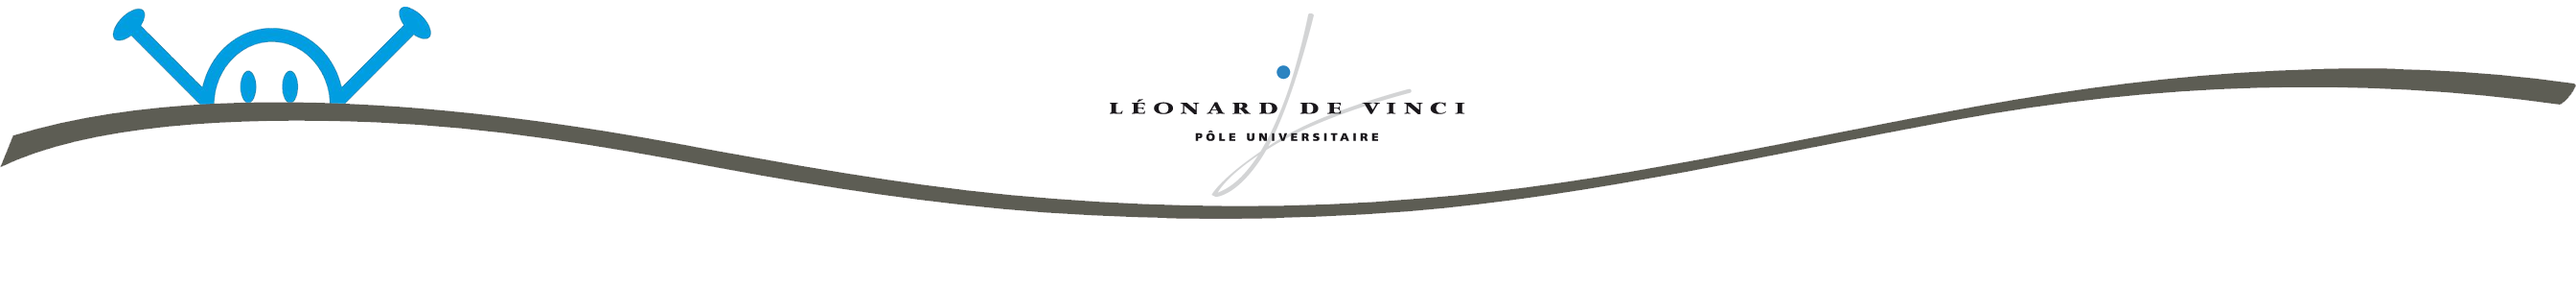
\includegraphics[width=\linewidth]{img_template/footer_titre.PNG}}
\rfoot{Page \thepage\ sur \pageref{LastPage}}
}

% ---- COLOR ---- %
\definecolor{gris}{rgb}{0.36,0.36,0.36}
\definecolor{bleu}{rgb}{0.1137,0.4941,0.5921}
\definecolor{gristitle}{rgb}{0.95,0.95,0.95}

\hypersetup{%
  colorlinks = true,
  linkcolor  = black,
  urlcolor = bleu 
}
%%%%%%%%%%%%%%%%%%%%%%%%%%%%%%%%%%%
% ---- Code dans le document ---- %
%%%%%%%%%%%%%%%%%%%%%%%%%%%%%%%%%%%
\usepackage{listings}

\lstset{
  basicstyle=\small\color{bleu},
  commentstyle=\color{gray},
}

%%%%%%%%%%%%%%%%%%%%%%%%%%%%%%%%%%%%%
\setlength{\parskip}{1em}
\renewcommand{\baselinestretch}{1.3}

%%%%%%%%%%%%%%%%%%%%%%%%%%%%%%%%%%%%%%%%%%%%%%%%%%%%%%%%%%%%%%%%%%%%%%%%%
%%%%%%%%%%%%%%%%%%%%%%%%%%%% PAGE DE GARDE %%%%%%%%%%%%%%%%%%%%%%%%%%%%%%
%%%%%%%%%%%%%%%%%%%%%%%%%%%%%%%%%%%%%%%%%%%%%%%%%%%%%%%%%%%%%%%%%%%%%%%%%

\begin{document}
\pagestyle{style}

\begin{center}
\begin{minipage}{0.75\linewidth}
\begin{center}
\centering
   
\vspace{3cm}
\colorbox{gristitle}{
\begin{minipage}{\textwidth}
    \begin{center}
    	\vspace{0.5cm}
    	%% Titre et sous titre 
    	{\color{bleu} \uppercase{\Huge {\titre}}}
    	\vspace{0.25cm}\linebreak
		\par \color{gris} {\Large \type}	
	\end{center}    
\end{minipage}    
}

\vspace{2.5cm}

% Description de Davincibot
\color{bleu} {\Large DaVinciBot \color{gris} : Association Robotique du pôle Léonard de Vinci  \par}
\end{center}

\vspace{1.5cm}
% Rapport redigé 
  
%Auteur
\color{gris} {\Large \textbf{Document rédigé par :}
\large
\begin{addmargin}[1em]{1em}
    \begin{itemize}[label= , noitemsep]
    	\auteur
    \end{itemize}
\end{addmargin}}
    
%Degree
\vspace{2.5cm}
%Date
\begin{center}
    {\large Dernière modification : \today \\ Document réalisé sous \LaTeX }
\end{center}
\end{minipage}
\end{center}

\newpage


%%%%%%%%%%%%%%%%%%%%%%%%%%%%%%%%%%%%%%%%%%%%%%%%%%%%%%%%%%%%%%%%%%%%%%%%%
%%%%%%%%%%%%%%%%%%%%%%%%%%%%%%%% CONTENU %%%%%%%%%%%%%%%%%%%%%%%%%%%%%%%%
%%%%%%%%%%%%%%%%%%%%%%%%%%%%%%%%%%%%%%%%%%%%%%%%%%%%%%%%%%%%%%%%%%%%%%%%%

\tableofcontents
\newpage

\section{Introduction}

\paragraph{DaVinciBot,} l'association de robotique de pôle Léonard De Vinci a développé une technologie de reconnaissance faciale pour le robot humanoïde InMoov.
Quatre étudiants en quatrième année de l'ESILV, école supérieure d'ingénieurs Léonard-de-Vinci, ont réalisé ce projet : 
\begin{itemize}
	\item Jérémy Martin
	\item Thomas Guillaume
	\item Chloé Mezouar 
	\item Aria Ekhteraei 
\end{itemize}
Leur objectif était de donner la possibilité au robot humanoïde InMoov, de pouvoir reconnaître la personne en face de lui et de pouvoir capter ses émotions pour adapté son comportement.\\
Dans ce document, nous vous présenterons comment mettre en place la reconnaissance faciale. \\
Vous pouvez retrouver plus d'info sur : \url{http://davincibot.org/inmoov-robot-cognitif/}

\section{Reconnaissance faciale}
\subsection{Pré-requis}

Pour pouvoir utiliser la reconnaissance faciale, il vous faudra plusieurs pré-requis :
\begin{itemize}
	\item Une caméra
	\item Un Ordinateur sous Linux (Ubuntu de préférence)
	\item Python 3.6 installé
\end{itemize}

Si vous n'avez pas la version de python 3.6 installée, je vous redirige vers ce tutoriel : 
\href{https://mk57blog.wordpress.com/2017/01/28/comment-modifier-la-version-par-defaut-de-python-sur-debian/}{Changer de version Python}

\subsection{Mise en place}

Avant tout, pour éviter le maximum de problèmes, je vous invite à installer l'IDE Python : Thonny. Pour cela, ouvrez l'interface Linux(Ctr + Alt + T) et tapez la commande suivante :
\begin{lstlisting}[language=bash]
  $ pip3 install thonny
\end{lstlisting}

Une fois installé, ouvrez cette IDE avec la commande :
\begin{lstlisting}[language=bash]
  $ thonny
\end{lstlisting}

Maintenant que nous sommes sur l'IDE Thonny, nous allons installé les librairies nécessaires, pour cela, allez dans "Tools" puis "Manage packages" et installez les packages suivant (certains peuvent prendre du temps): 
\begin{itemize}
	\item[•] opencv-python
	\item[•] numpy
	\item[•] scipy
	\item[•] scikit-image (Ce n'est pas dérangeant si un message d'erreur apparaît)
 	\item[•] dlib
	\item[•] face\_ recognition
	\item[•] easygui
\end{itemize}

Ensuite, créez un nouveau dossier dans votre ordinateur.\\
Dans ce dernier placez-y le script python "Face Recongnition V3.py" que vous pouvez télécharger sur ce GitHub : \href{https://github.com/MadScientistHK/Pi2_Face_Recognition}{Script python}\\
Puis dans le même dossier, vous allez en créer un nouveau que vous appellerez "Pi2".\\
Et à l'intérieur de celui-ci, créez un dernier dossier appelé "tmp\_ dataset"
\vspace{1cm}
\\
Cela étant fait, nous pouvons retourner sur l'IDE Thonny, ouvrir le script "Face Recognition V3.py", et lancez le.


\subsection{Utilisation}

Une fois le script python exécuté, une fenêtre devrait apparaître montrant ce que capte la caméra de l'ordinateur. Dès qu'un visage apparaît devant cette dernière, il est reconnu et entouré d'un carré bleu indiquant le nom de la personne ou un "unknow" si cette personne n'est pas enregistrée dans la base de donnée. \\
Pour ajouter une nouvelle personne, deux options s'offrent à vous:\\
Soit vous attendez le message, appuyez sur "oui" puis rentrez son nom.\\
Soit vous la prenez directement en photo et ajouter cette dernière dans le dossier  "tmp\_ dataset".

\paragraph{ATTENTION} Il ne faut jamais mettre deux fois le même nom et il ne faut qu'un seul visage visible sur chaque photo!
\vspace{1cm}

\newpage
Si vous voulez maintenant utiliser une caméra externe, deux options s'offrent à vous:\\
Soit vous pouvez désactiver les drivers de votre caméra avec une touche. \\
Soit vous modifier la ligne de code ci-dessous en remplaçant le "0" par un "1" :
\begin{lstlisting}[language=bash]
  cap = videocapture(0) 
\end{lstlisting}

\section{Conclusion}
Merci d'avoir pris connaissance de ce tutoriel, pour plus de renseignements sur nos différents projet en lien avec inMoov, rendez-vous sur le site de DaVinciBot : \href{http://davincibot.org/inmoov/}{DaVinciBot - InMoov} \\
Bonne continuation !

\vspace{2cm}
\begin{center}
	
\includegraphics[width = 10cm]{Images/DaVinciBot_Square.png}
\end{center}

\end{document}